\section{Study2: relationship between stress-buffering effect of automatically extracted positive events and microblog characteristics}

\subsection{Positive events automatically extracted from microblogs}
Since events in study 1 are scheduled and limited,
in this part we first introduce the procedure to extract positive event and its intervals from microblogs,
thus to extend our study to various types of positive events expressed in microblogs.
%Our automatically extraction accuracy was verified
%by comparing extracted positive events with scheduled school events in coincident time intervals.

\paragraph{Linguistic structure}
Let $u$ = $[type,\{doer, act,$ $description\}]$ be a positive event,
where the element \emph{doer} is the subject who performs the \emph{act},
and \emph{descriptions} are the key words related to $u$.
According to psychological scales \citep{hassles,Jun2008Influence},
adolescents' positive events mainly focus on six aspects,
as $\mathbb{U} =\{$ 'entertainment', 'school life', 'romantic', 'pear relationship', 'self-cognition', 'family life'$\}$.
% $\forall u$, $u._{type} \in \mathbb{U}$.
%Similar to positive event,
%let $e$ = $[type,\{role, act,$ $descriptions\}]$ be a stressor event.
%According to psychological questionnaires \cite{scale2, scale3, Kanner1981Comparison, scale1},
%we classify stressor events into five types, as $\mathbb{S}=\{$ \emph{'school life', 'family life',
%'pear relation', 'self-cognition', 'romantic'}$\}$, $\forall e$, $e._{type} \in \mathbb{S}$.

\paragraph{Lexicon}
We constructed our lexicon for six-dimensional positive events from two sources.
The basic positive words are selected from the psychological lexicon SC-LIWC (e.g., \emph{expectation}, \emph{joy}, \emph{love} and \emph{surprise})~\citep{Tausczik2010The}.
Then we built six topic lexicons by expanding basic positive words from adolescent microblogs,
containing 452 phrases in 'entertainment',
273 phrases in 'school life',
138 phrases in 'romantic',
91 phrases in 'peer relationship',
299 phrases in 'self-recognition' and 184 phrases in 'family life', with totally 2,606 phrases,
as examples shown in table \ref{tab:keyWords}.
Additionally, we labeled \emph{doer} words (i.e., \emph{teacher}, \emph{mother}, \emph{I, we}) in the positive lexicon.

\paragraph{Parser relationship}
For each post, after word segmentation, we parsed current sentence to find its linguistic structure,
and then matched the main linguistic components with positive topic lexicon in each dimension.
The parser model in Chinese natural language processing platform \citep{Che2010} was adopted in this part,
which identified the central verb of current sentence first, namely the \emph{act},
and constructed the relationship between the central verb and corresponding \emph{doer} and \emph{description} components.
By searching these main elements in positive event related lexicons,
we identified the existence and type of positive events.
Due to the sparsity of posts, \emph{act} might be empty.
\emph{Descriptions} were collected by searching all nouns, adjectives and adverbs.
In such way, we extracted structured positive events from microblogs.

Examples of adolescents' microblogs describing positive events are listed in table \ref{tab:uplifts}.
For the post 'Thanks all my dear friends hosting the party. Happiest birthday!!!',
we translated it into \emph{doer='friends', act = 'expecting', description = 'party'},
and \emph{type = 'entertainment'}.
To check the accuracy of positive event extraction,
in study 3,
we identified positive events and its corresponding stress-buffering effect from microblogs,
and compared the results with positive events in school planning.

\begin{table}
\begin{center}
\caption{\small{Structured extraction of positive events from microblogs.}}
\small{
\begin{tabular}{l} \hline \rowcolor{gray!40}
I am really looking forward to the spring outing on Sunday now. \\ \rowcolor{gray!40}
(doer:\emph{I}, act:\emph{looking forward}, description:\emph{spring outing})\\
My holiday is finally coming [smile]. \\
(doer:\emph{My holiday}, act:\emph{coming}, description:\emph{[smile]})\\ \rowcolor{gray!40}%\hline
First place in my lovely math exam!!! In memory of it.\\ \rowcolor{gray!40}
(description:\emph{first place, math, exam, memory})\\ %\hline
You are always here for me like sunshine. \\
(doer:\emph{You}, description:\emph{sunshine})\\ \rowcolor{gray!40} %\hline
Thanks all my dear friends hosting the party.
Happiest birthday!!!\\ \rowcolor{gray!40}
(doer:\emph{friends}, act:\emph{thanks}, description:\emph{party, birthday})\\
I know my mom is the one who support me forever, no matter \\
when and where. (doer:\emph{mom}, act:\emph{support})\\ \rowcolor{gray!40}
Expecting Tomorrow' Adult Ceremony[Smile][Smile]~~\\ \rowcolor{gray!40}
(act: \emph{expecting}, description:\emph{Adult Ceremony})\\ \hline
\end{tabular}}
\label{tab:uplifts}
\end{center}
\end{table}

\paragraph{Impact Interval of Positive Event}
Next, we identified the impact interval of each positive event thus to further study its stress-buffering pattern.
Splitting interval is a common time series problem, and here we identified the target interval in three steps.
In the first step, we extracted positive events, stressor events~\citep{Li2017Analyzing} and filtered out candidate intervals after a smoothing process.
Since the stress series detected from microblogs were discrete points,
the loess method was adopted to highlight characteristics of the stress curve (see \ref{alg:alg1}).
In the second step, applying the Poisson based statistical method~\citep{Li2017Analyzing},
we judged whether each candidate interval was a confidential stressful interval.
Finally, we divided the stressful intervals into two sets: the SI set and the U-SI set,
according to its temporal order with neighboring positive events (see \ref{alg:alg2}).


\subsection{Measures}
\label{measures}
We examined the relationship
between positive events and stress-buffering pattern through three groups of measures:
posting behavior, stress intensity, and linguistic expressions.

\textbf{Posting behaviors}.
Stress could lead to abnormal posting behaviors,
reflecting user's changes in social engagement activity ~\citep{Liang2015Teenagers}.
In this study,
we considered four measures of posting behaviors in each time unit (day),
and presented each measure as a corresponding series.
The first measure was \emph{posting frequency},
representing the total number of posts per day.
Research in \cite{Li2017Analyzing} indicated that overwhelmed adolescents tended to post more to express their stress for releasing
and seeking comfort from friends.
The second measure \emph{stressful posting frequency} per day
was based on existing stress detection result and highlights the stressful posts among all posts.
The third measure was the \emph{positive posting frequency}, indicating the number of positive posts per day.
The forth measure \emph{original frequency} was the number of original posts, which filters out re-tweet and shared posts.
Compared to forwarded posts, original posts indicated higher probability that users were talking about themselves.
Thus in each interval, user's posting behavior was represented as a four-dimension vector.

\textbf{Stress change mode}.
The global stress change mode during a stressful interval was depicted through four measures:
\emph{sequential stress level, length, RMS,} and \emph{peak}.
Basically, \emph{stress level} per day constructed a sequential measure during a stressful interval,
recording stress values and fluctuation on each time point.
As positive events might conduct impact on stressed adolescents,
and postpone the beginning or promote the end of a stressful interval,
we took \emph{length} as the second factor representing the interval stress change mode.
To quantify the intensity of stress fluctuations,
\emph{RMS} (root mean square) of stress values through the interval was adopted  as the third measure.
\emph{Peak} value was adopted as the forth measure to show the maximal stress value in current interval.

\textbf{Linguistic expressions}.
Positive and stressful expressions were extracted from the post content.
The first linguistic measure was the frequency of \emph{positive word},
which represented the positive emotion in current interval.
The second measure was the frequency of \emph{positive event topic words} in six dimensions,
reflecting the existence of positive events.
\citep{Li2014Major} showed that self-mentioned words showed high probability that the current stressor event was related to the author,
rather than the opinion about a public event or life events about others.
Another important factor was wether existing \emph{self-mentioned words} (i.e., \emph{'I','we','my'}).
Except positive-related linguistic descriptions, we also took stressful linguistic characters as measures,
while also offered information from the complementary perspective.
The frequency of \emph{stressor event topic words} in five dimensions represented the degree of attention for each type of stressor event.
The frequency of \emph{pressure words} reflected the degree of general stress emotion during the interval.

Next,
based on the above measures,
we quantified the difference between SI and U-SI sets, thus to track the stress-buffering pattern of positive events.

\begin{figure*}
\centering
\includegraphics[width=0.9\linewidth]{figs/BOX3.eps}%figs/correlation2.eps
\caption{Stress-buffering pattern of positive events. Figure a) shows correlation of each microblog measure,
and figure b) shows stress-buffering effect on five dimensions of stress. 'KTS' means KNN-based correlation method.}
\label{fig:correlation}
\end{figure*}

\subsection{Method}
In our problem,
there were two sets of stressful intervals to compare:
the SI set and the U-SI set,
containing stressful intervals not affected by positive events
and stressful intervals impacted by positive events, respectively.
The basic elements in each set were stressful intervals.
Each interval was modeled as a multi-dimensional vector according to the three groups of measures in section ~\ref{measures}.
Thus we formulated this comparison problem as finding the correlation between the two sets of multi-dimension points.
Specifically, we adopted the multivariate two-sample hypothesis testing method
\cite{Li2017Correlating,Johnson2012Applied} to model such correlation.
In this two-sample hypothesis test problem,
the basic idea is judging whether the multi-dimension points (i.e., stressful intervals)
in set SI and set U-SI were under different statistical distribution.
Assuming the data points in SI and U-SI were randomly sampled from distribution $F$ and $G$, respectively,
then the hypothesis was denoted as:
\begin{equation}
H_0: F = G \quad versus \quad H_1: F \neq G.
\end{equation}

Under such hypothesis,
$H_0$ indicates points in SI and U-SI were under similar distribution,
while $H_1$ means points in SI and U-SI were under statistically different distributions,
namely positive events conducted obvious stress-buffering effect on current user.
Since each point in the two sets (SI and U-SI) was depicted in multi-dimensions,
here we took the KNN (K-Nearest Neighbor) \cite{Schilling1986Multivariate}
based method to judge the existence of significant difference between SI and U-SI.
For simplify, we used the symbol $A_1$ to represent set SI,
and $A_2$ represent set U-SI.
In the KNN algorithm,
for each point $\ell_{x}$ in the two sets $A_1$ and $A_2$,
we expected its nearest neighbors (\emph{the most similar points}) belonging to the same set of $\ell_x$.
The model derivation process was presented in ~\ref{mod:mod1}.

\subsection{Results}
\paragraph{Stress-buffering Pattern of scheduled positive events}
Basically, we focused on four scheduled positive events:
\emph{practical activity}, \emph{holiday}, \emph{new year party} and \emph{sports meeting}.
For each of the four scheduled positive events,
we quantified the stress-buffering effect based on corresponding SI and U-SI interval sets of the 124 students.

\begin{table}[H]
\begin{center}
\caption{\small{Quantify the impact of scheduled positive school events using KTS (the KNN-based two sample method adopted in this research) and baseline method.}}
\label{tab:schedule}
\resizebox{0.45\textwidth}{13mm}{
\small{
\begin{tabular}{lccccc}
\toprule
&	\emph{practical}	&	         	&	\emph{new year}	&	\emph{sports}	&	\emph{}	\\
&	\emph{activity}	&	\emph{holiday}	&	\emph{party}	&	\emph{meeting}	&	\emph{all}	\\
\midrule
size of U-SI	&	219 	&	339 	&	235 	&	226 	&	1,019 	\\
Pearson         &55.65\%	&	70.97\%	&	56.45\%	&	54.84\%	&	65.32\% \\
KTS             &54.52\%	&	78.39\%	&	63.39\%	&	58.74\%	&	69.52\% \\
\bottomrule
\end{tabular}
}
}
\end{center}
\end{table}

Table \ref{tab:schedule} shows the experimental results,
where 54.52\%, 78.39\%, 63.39\%, 58.74\% significant stress-buffering effect were detected for the four specific scheduled positive events,
with the total ratio to 69.52\% ($\alpha$ =1.96 for p=0.025).
We adopted the commonly used Pearson correlation algorithm to compare with the two sample statistical method in this study.
The Euclidean metric was used to calculate the distance between two $n$ dimension points $X$ and $Y$.
Experimental results show that our KNN-based two sample method (denoted as KTS) outperformed the baseline method
with the best improvement in \emph{new year party} to 10.94\%,
and total improvement to 6.00\%.


\begin{table*}
\begin{center}
\caption{\small{Monotonous stress intensity changes in U-SI and SI intervals compared with adjacent intervals.}}
%\resizebox{\textwidth}{15mm}{
\small{
\begin{tabular}{l cccccc cccccc} \\\hline\hline
\multirow{2}{1cm}{}
&\multicolumn{2}{c}{school life}
&\multicolumn{2}{c}{romantic}
&\multicolumn{2}{c}{peer relationship}
&\multicolumn{2}{c}{self-cognition}
&\multicolumn{2}{c}{family life}
&\multicolumn{2}{c}{all types}\\
&U-SI	    &	SI	        &U-SI	    &SI	        &U-SI	   &SI	
&U-SI	    &	SI	        &	U-SI	&SI	        &U-SI	   &SI\\  \hline
\# interval         &   365	        &	514	        &	536	        &	587	        &128	    &	391	        &	564	           &	609	            &	321	        &	481	        &	1,914	    &2,582	 \\
front $\rightarrow$ I &	72.60\% &	78.79\% &	69.03\% 	&77.51\%   &74.22\%    &81.59\%    &70.04\%    &77.67\%  &67.91\%     &77.96\%    &70.17\%    &78.51\% \\
I $\rightarrow$ rear  &	75.89\% &	78.40\% &	74.63\% 	&79.05\%   &78.13\%    &82.61\%    &75.00\%    &79.15\%   &74.14\%    &79.42\%    &75.13\%    & 79.55\%\\ \hline \hline
\end{tabular}}%}}
\label{tab:fontrear}
\end{center}
\end{table*}

The correlation of positive events a) in each group of microblog measure
and b) towards five dimensions of stress
were shown in box-plots \ref{fig:correlation}.
The stress-buffering pattern of positive events
was closely correlated with posting behavior (ratio = 80.65\%, n=100, SD=1.96),
stress change mode (ratio = 67.74\%, n=84, SD=2.04) and microblog linguistic expressions (ratio = 74.19\%, n=92, SD=2.07).
Positive events conducted most intensive stress-buffering impact on 'family life' (ratio = 83.87\%, n=104, SD=2.72),
followed by 'peer relationships' (ratio = 71.77\%, n=89, SD=4.04) and 'school life' (ratio = 67.74\%, n=84, SD=2.71) dimensions.
The correlation values in 'peer relation'
exhibited the highest 75th percentile while the lowest 25th percentile,
showing a relatively random and unstable stress-buffering effect on this dimension.
Comparing the hypothesis test results on scheduled positive events (ratio = 69.52\%)
and automatically extracted positive events (ratio = 74.21\%),
the result indicated the feasibility of automatically extracting positive events from microblogs.

\section{Study3: Testing the monotonous stress changes of stress-buffering from adolescents' microblogs}
\subsection{Method}
To verify the monotonous stress changes at both the early and late stress-buffering stages,
for each stressful interval in SI (n=2,582) and U-SI (n=1,914),
we compared its stress intensity with the front and rear adjacent intervals using t-test method.
Detailed algorithms are presented in \ref{mod:mod2}.

\subsection{Result}
Here four situations were considered and compared,
as shown in table \ref{tab:fontrear}.
The \emph{ratio of intervals} detected with monotonous increase from the \emph{front interval} to \emph{stressful interval} (denoted as \emph{front$ \rightarrow$ I}),
and monotonous decrease from the \emph{stressful interval} to the \emph{rear interval} (denoted as \emph{I $\rightarrow$ rear}) were listed.
Under the effect of positive events,
the ratio of intensive stress increase in \emph{front$ \rightarrow$ I} was decreased from 78.51\% to 70.17\%;
and the ratio of intensive stress decrease in \emph{I $\rightarrow$ rear} was decreased from 79.55\% to 75.13\%.
The most obvious monotonous decrease in \emph{front$ \rightarrow$ I} were conducted by positive events in family life dimension (12.89\% reduction);
and the most obvious monotonous decrease in \emph{front$ \rightarrow$ I} were also conducted by positive events in family life dimension (6.65\% reduction).
The experimental results indicated the effectiveness of the two sample method for quantifying the effect of positive events,
and the rationality of the assumption that positive events could help ease stress of overwhelmed teens.
